
\section{Division}

We will review division in this lesson. Division is used when we divide a number evenly into certain groups. Look at this figure:
\\[0.1in]
\begin{tightcenter}
   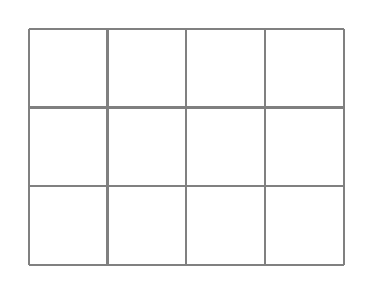
\begin{tikzpicture}
      \draw[step=1.0cm,gray,thick]
      (0,0) grid (4,3);
   \end{tikzpicture}
   \captionof{figure}{a $4$ by $3$ grid}
   \label{fig:grid}
\end{tightcenter}

There are a total of $12$ blocks. If we divide them into $3$ rows, each row would have $12 \div 3 = 4$ blocks.

If we divide $12$ blocks into $4$ columns, each column would have $12 \div 4 = 3$ blocks.

A second way to understand division is to "repeatedly take way." Assume there are $12$ blocks. If $3$ blocks are taken away each time, it will take $12 \div 3 = 4$ turns to take away all $12$ blocks.

In $12 \div 3 = 4$, we call the result $4$ the \textit{quotient} of $12$ and $3$. Earlier, we learned the words \textit{sum}, \textit{difference} and \textit{product}. Please memorize the meaning of these $4$ words. For example, when if you see the word \textit{product}, you know you are dealing with multiplication.

\subsection{Multiplication and Division}

Multiplication and division are \textit{inverse operations}. For example:
\begin{itemize}
\item $12 \div 3 = 4$ as $3 \cdot 4 = 12$
\item $15 \div 3 = 5$ as $3 \cdot 5 = 15$
\item $0 \div 3 = 0$ as $3 \cdot 0 = 0$
\end{itemize}

This explains why we cannot "divide by $0$". Let's look at:
\[ 3 \div 0 \]
Assume we can do this, and we have 
\[ 3 \div 0 = \text{some number} \] 
Since multiplication and division are inverse operations, we have:
\[ 0 \cdot \text{some number} = 3 \]

We know $0$ times any number is always $0$, so there is no way we can find a number which makes $0 \cdot \text{some number} = 3$ work. This is why we cannot divide a number by $0$. Notice the difference:

\[
0 \div 3 = 0 \text{ while } 3 \div 0 = \text{undefined}
\]

If you do $3 \div 0$ on a calculator, you will receive an error.

\subsection{Multiplication and Division Symbols}
We are used to using the multiplication and division symbols we learned from grade school, as in $3 \times 4 = 12$ and $12 \div 3 = 4$.

Starting now, we will use $\cdot$ to represent multiplication, and use the fraction line to represent division. For example:

\[ 3 \cdot 4 = 12 \text{ and } \frac{12}{3}=4 \]

The fraction line simply means division. Once you understand this, you will understand fractions better.

\subsection{Division Word Problems}
Next, let's look at some examples where division is used. There are two situations where division is needed:
\begin{enumerate}
  \item dividing a number evenly into groups, and
  \item repeatedly taking away
\end{enumerate}

\begin{myexample}
	A teacher will do a math activity in a class. She will hand out $56$ blocks to $8$ students. If each student receives the same number of blocks, how many blocks will each student get?
\label{ex:blockDivision}
\end{myexample}
\begin{solution}
	In this problem, we need to divide $56$ blocks evenly into $8$ groups. Each student will get $\frac{56}{8}=7$\ blocks.
\end{solution}

\begin{myexample}
   Omar bought $48$ M\&M candies, and plans to eat $4$ of them every day. How many days will these candies last?
\label{ex:MMDivision}
\end{myexample}
\begin{solution}
	In this problem, we need to repeatedly take away $4$ candies from $48$ candies. This is a division problem. These candies will last $\frac{48}{4}=12$ days.
\end{solution}

\subsection{Remainder}
Let's learn remainder in context.
\begin{myexample}
	A teacher will do a math activity in a class. She will hand out $60$ blocks to $8$ students. If each student receives the same number of blocks, how many blocks will each student get?
\label{ex:BlockDivisionRemainder}
\end{myexample}
\begin{solution}
This example is very similar to \cref{ex:blockDivision}. However, we get a decimal quotient if we do $\frac{60}{8}=7.5$. In this context, it's unlikely that the teacher will break up blocks and hand out half of a block to students. Each student will still get $7$ blocks.

If each student gets $7$ blocks, a total of $7 \cdot 8=56$ blocks will be handed out. The remainder is $60-56=4$, implying $4$ blocks will be left.

\textbf{Conclusion:} Each student will get $7$ blocks, with $4$ blocks left.
\end{solution}

\begin{myexample}
	A teacher will do a math activity in a class. She will put all $60$ blocks into containers. Each container can hold $8$ blocks. How many containers will be needed?
\label{ex:MMDivisionRemainder}
\end{myexample}
\begin{solution}
Compare this with \cref{ex:BlockDivisionRemainder}. We still do $\frac{60}{8}=7.5$, but the context is different. The quotient is $7.5$, implying we need $8$ containers to hold $60$ blocks, but the last container is not full.

If each container holds $8$ blocks, $7$ containers can hold a total of $7 \cdot 8=56$ blocks. The remainder is $60-56=4$, implying the last container is not full, holding $4$ blocks.

\textbf{Conclusion:} $8$ containers are needed, with the last container holding $4$ blocks.
\end{solution}

Note that we didn't use long-division to find remainders. Especially for big numbers, we will use a calculator, instead.

\begin{myexample}
Find the remainder of $\frac{121}{7}$ without doing long division.
\label{ex:findRemainder}
\end{myexample}
\begin{solution}
To find the remainder of $\frac{121}{7}$, the calculator tells us $\frac{121}{7}=17.285714...$, implying the quotient is $17$. This means, if we divide $121$ blocks into groups of $7$ blocks, there will be $17$ groups, with some leftover. These $17$ groups have $7 \cdot 17 = 119$ blocks, and the remainder is $121-119=2$.
\end{solution}

We need this skill later to change an improper fraction to a mixed number, as in
\[ \frac{121}{7}=17 \frac{2}{7} \]

\subsection{Summary}
Let's review important concepts in this lesson.
\begin{itemize}
\item Division is used when we divide a number evenly into groups, and when we repeatedly take away a smaller number from a bigger number.
\item The result of division is called the quotient.
\item Instead of using the division symbol $\div$, we can use the fraction line, as in $\frac{6}{2}=3$.
\item We can find the remainder without using long division, as in \cref{ex:findRemainder}.
\end{itemize}
